\mysubsection{Correlated versus uncorrelated n-n energy distribution}
\label{sec:n_n_erg_dist}
In order to effectively minimize the dependence of the result on detector geometry/efficiency, the numerator and denominator of Eq.~\ref{eq:angularCorr} must comprise neutron pairs with a similar energy distribution.
Note that accidental coincident neutrons from $(\gamma,n)$ are completely removed from $nn_{\text{corr}}(\theta)$, the numerator in Eq.~\ref{eq:angularCorr}, by the subtraction of accidental coincidences, but are not removed from the denominator, $nn_{\text{uncorr}}(\theta)$.
This is the reason for using only pulse-pairs that have two events in each pulse when determining the uncorrelated neutron distribution.
Doing so increases the selection of neutrons from fission as opposed to $(\gamma,n)$. 
%accidental coincidence neutrons from fission and $(\gamma,n)$ have different energy distributions, and 

When examining differences between the neutron energy distributions in $nn_{\text{corr}}(\theta)$ and $nn_{\text{uncorr}}(\theta)$, it is important to consider how the energies of both neutrons forming n-n pairs vary together, or, in other words, their joint energy distribution.
Figure~\ref{fig:ErgDiffLego} shows the ratio between the rates for correlated and uncorrelated n-n pairs of various binned energies.
The effect that these discrepancies in energy distribution have on the final result can be examined by applying a weighting factor to each event in $nn_{\text{uncorr}}(\theta)$ such that a recalculation of the result in Fig.~\ref{fig:ErgDiffLego} produces a flat curve.
A comparison of the angular correlation with and without the application of these weighting factors to uncorrelated n-n events is seen in Fig.~\ref{fig:WeightedErgDiff}.
The resulting angular correlations are identical to within experimental uncertainties, suggesting that differences in the energy distributions of $nn_{\text{corr}}(\theta)$ and $nn_{\text{uncorr}}(\theta)$ do not significantly affect the present measurement.
\begin{figure}[]
\centering
    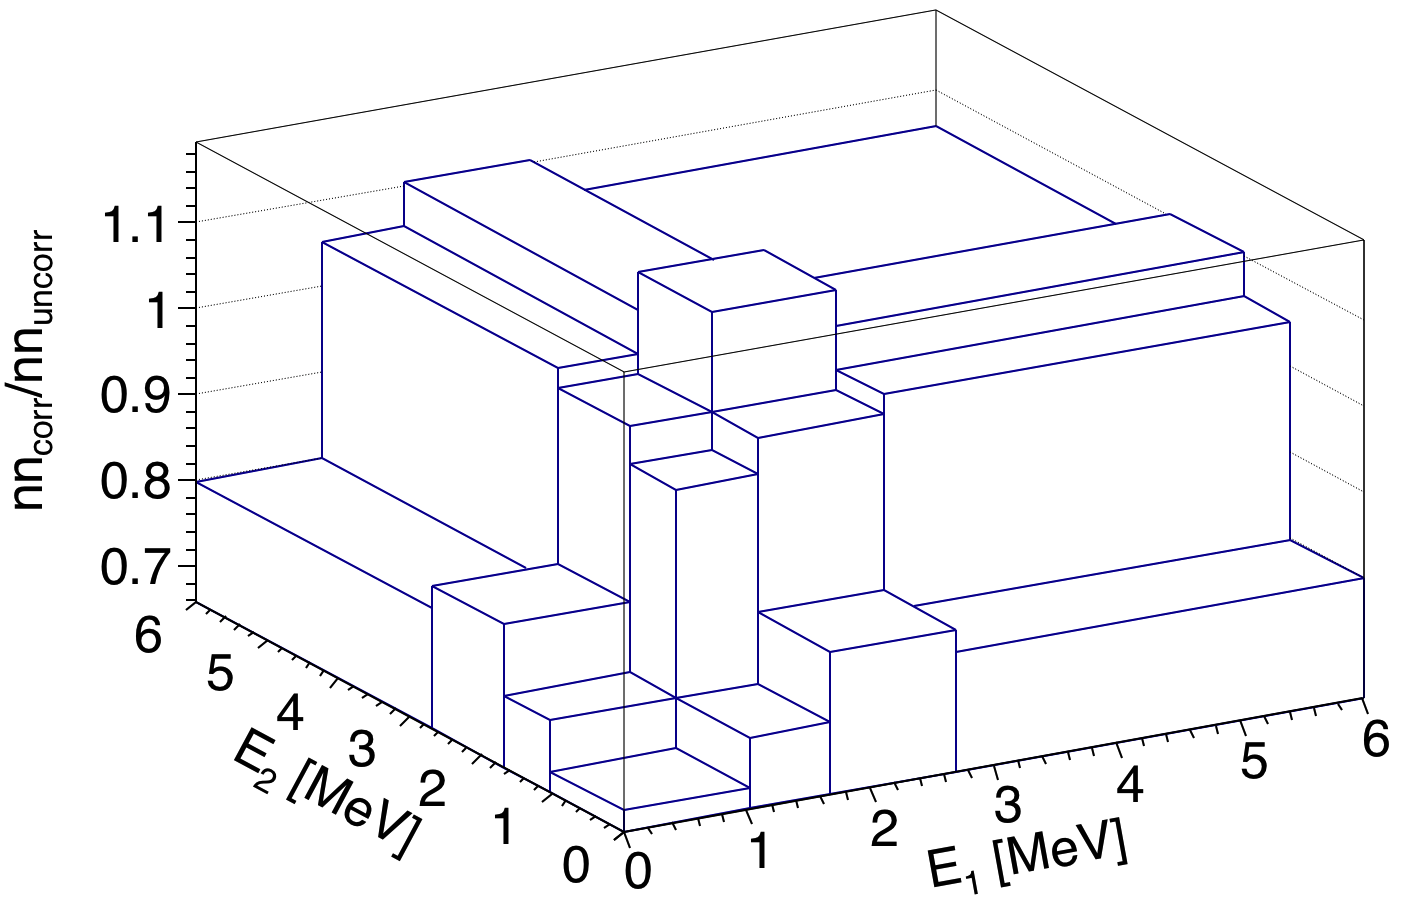
\includegraphics[width=\figsize\textwidth]{ErgDiffLego.png}
    \caption{
    The z-axis represents the ratio between the correlated and uncorrelated rates of binned n-n energies.
    The energy bins are chosen such that each contains an equal number of events, or 1/16th of the total events.
    }
    \label{fig:ErgDiffLego}
\end{figure}
\begin{figure}[]
\centering
    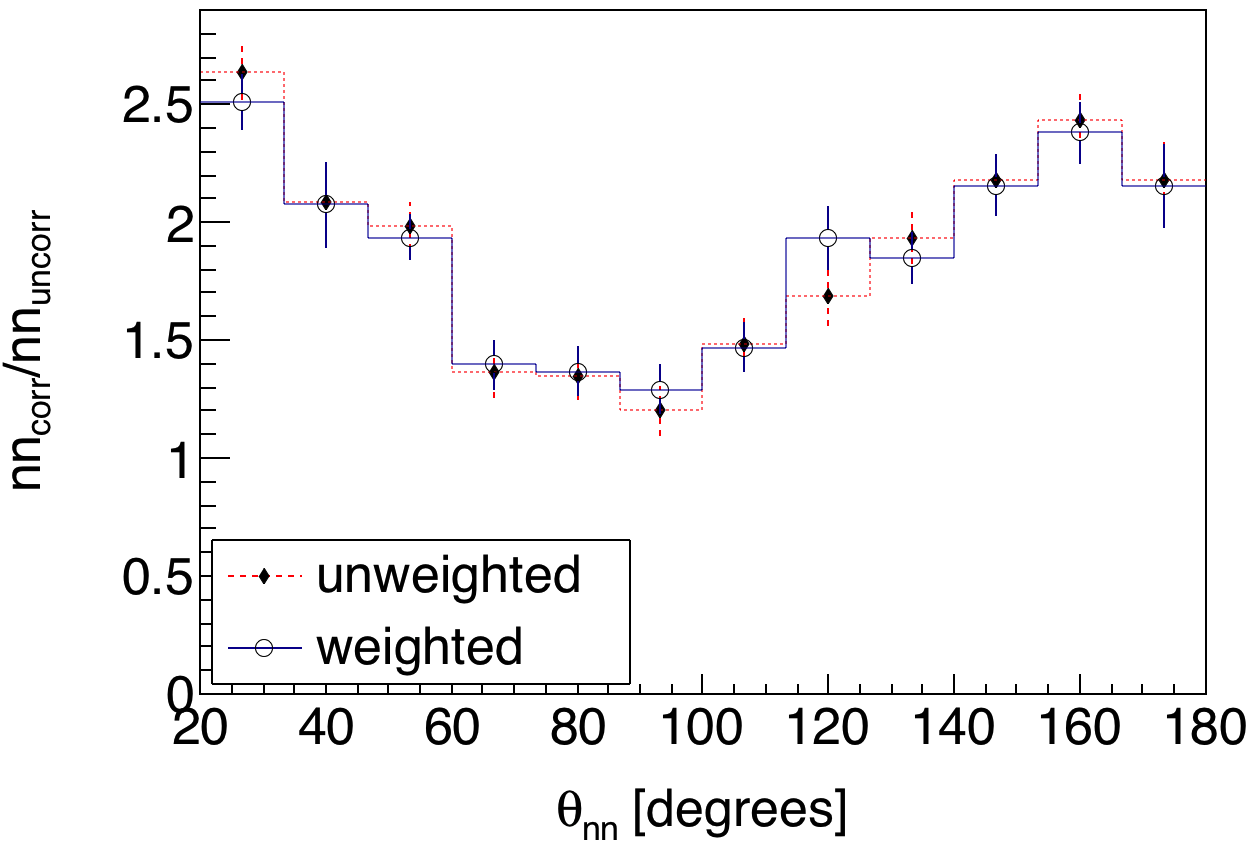
\includegraphics[width=\figsize\textwidth]{WeightedErgDiff.png}
    \caption{
Each uncorrelated n-n event can be weighted such that the weighted histograms of the joint n-n energy distributions of correlated and uncorrelated n-n pairs are equal.
Comparison of the calculated angular correlation results, with and without such weighting factors applied to all uncorrelated n-n events, illustrates that any effects due to the discrepancies in the joint energy distributions of correlated and uncorrelated n-n pairs are negligible.
    }
    \label{fig:WeightedErgDiff}
\end{figure}

\mysubsection{Detector Cross-talk}
\label{crosstalk}
\textit{Cross-talk} occurs when, after a particle is detected once, the same particle, by any means, causes a detection to be registered in a different detector.
For example, upon detection, a particle may undergo elastic scattering and then travel into another detector where it is detected again, or, it may produce secondary particles that are detected.
The two coincident detections of a cross-talk event are causally correlated, and thus they have the potential to contaminate the signal from correlated fission neutrons.
If both detections occur during the ToF range typical for fission neutrons, then the cross-talk event cannot be distinguished from the detection of two correlated neutrons.

Recent works that measured the n-n angular correlations in the spontaneous fission of $^{252}$Cf and $^{240}$Pu~\cite{Pozzi2016,Verbeke2018} addressed this effect by using an MCNP-PoLiMi simulation to estimate and then subtract cross-talk from their measurements.
In this work, the issue of cross-talk is approached differently by employing the use of detector shielding aimed at reducing cross-talk to a negligible rate.
By using shielding to reduce cross-talk, this measurement is less dependent on the details of the models used by MCNP-PoLiMi to simulate neutron transport and detection.
MCNP-PoLiMi simulations are used in this work only to verify that the effect of cross-talk is negligible.

The scintillators used here are much larger than those used in similar works, such as in Refs.~\cite{Pozzi2016,Verbeke2018}, allowing them to be placed much farther from the fission source without causing a detrimental loss in coincidence rates. 
An increase in the distance between the detectors and the fission source makes this measurement less subject to to angular uncertainty, which depends directly on the uncertainty in the position of a detected particle due to, for example, the scattering of neutrons from detector shielding.
For this reason, larger amounts of shielding can be used without concern of introducing large errors.
 
Furthermore, the geometry of the neutron detection system makes it kinematically impossible for a neutron to undergo a single scattering event with a proton in one detector, which is the basis for scintillation, and then travel directly into another detector with enough kinetic energy to be detected a second time.
For this reason, upon being detected, a neutron must scatter from one or more intermediate nuclei, such as lead or carbon, in order for it to reach another detector with enough energy to be detected again.
This fact follows from the conservation of energy and momentum.
In order to support the claim that the design of the neutron detection system reduced cross-talk to negligible rates, a detailed MCNP-PoliMi~\cite{MCNP_POLIMI} simulation was performed in which a built-in $^{252}$Cf source is positioned at the center of a model of the neutron detection system.

\mysubsubsection{Simulation of Detector Cross-talk}
The cross-talk simulation included all scintillators, shielding, detector supporting structures, and the concrete walls surrounding the experimental cell.
MCNP-PoliMi's built-in $^{252}$Cf spontaneous fission source was used, which emits neutrons with the correct correlations and multiplicities according to previous measurements.
Detector response was modeled using a program included with the MCNP-PoliMi distribution called MPPost~\cite{MPPost}.
The model is based on the MeV electron equivalent (MeVee) light output produced by particles as they undergo collisions with carbon and hydrogen within organic plastic scintillators.
A minimum deposited energy of 0.4 MeV (equivalent to 0.05 MeVee for neutrons) was assumed for detectable particles, which was chosen because the neutron detection system exhibited a sharp decline in detection efficiency for neutrons below 0.4 MeV.

For neutron collisions with hydrogen, the light output in MeVee, denoted $L$, is calculated by the following empirically derived formula~\cite{MPPost}
\begin{displaymath}
L = 0.0364 \Delta E_n^2 +  0.125 \Delta E_n \, ,
\end{displaymath}
where $\Delta E_n$ is equal to the loss in the kinetic energy of the neutron due to the collision.
Neutron interactions with carbon are assumed to generate a small light output of
\begin{displaymath}
L = 0.02 \Delta E_n \, .
\end{displaymath}
As seen in Fig.~\ref{fig:Cf252MCNPVsEXP}, this model of the detection process produces a ToF spectrum for the SF of $^{252}$Cf that shows good agreement with the measurement for neutrons with a ToF less than 100 ns and fair agreement for neutrons with a ToF greater than 100 ns.
\begin{figure}
    \centering
    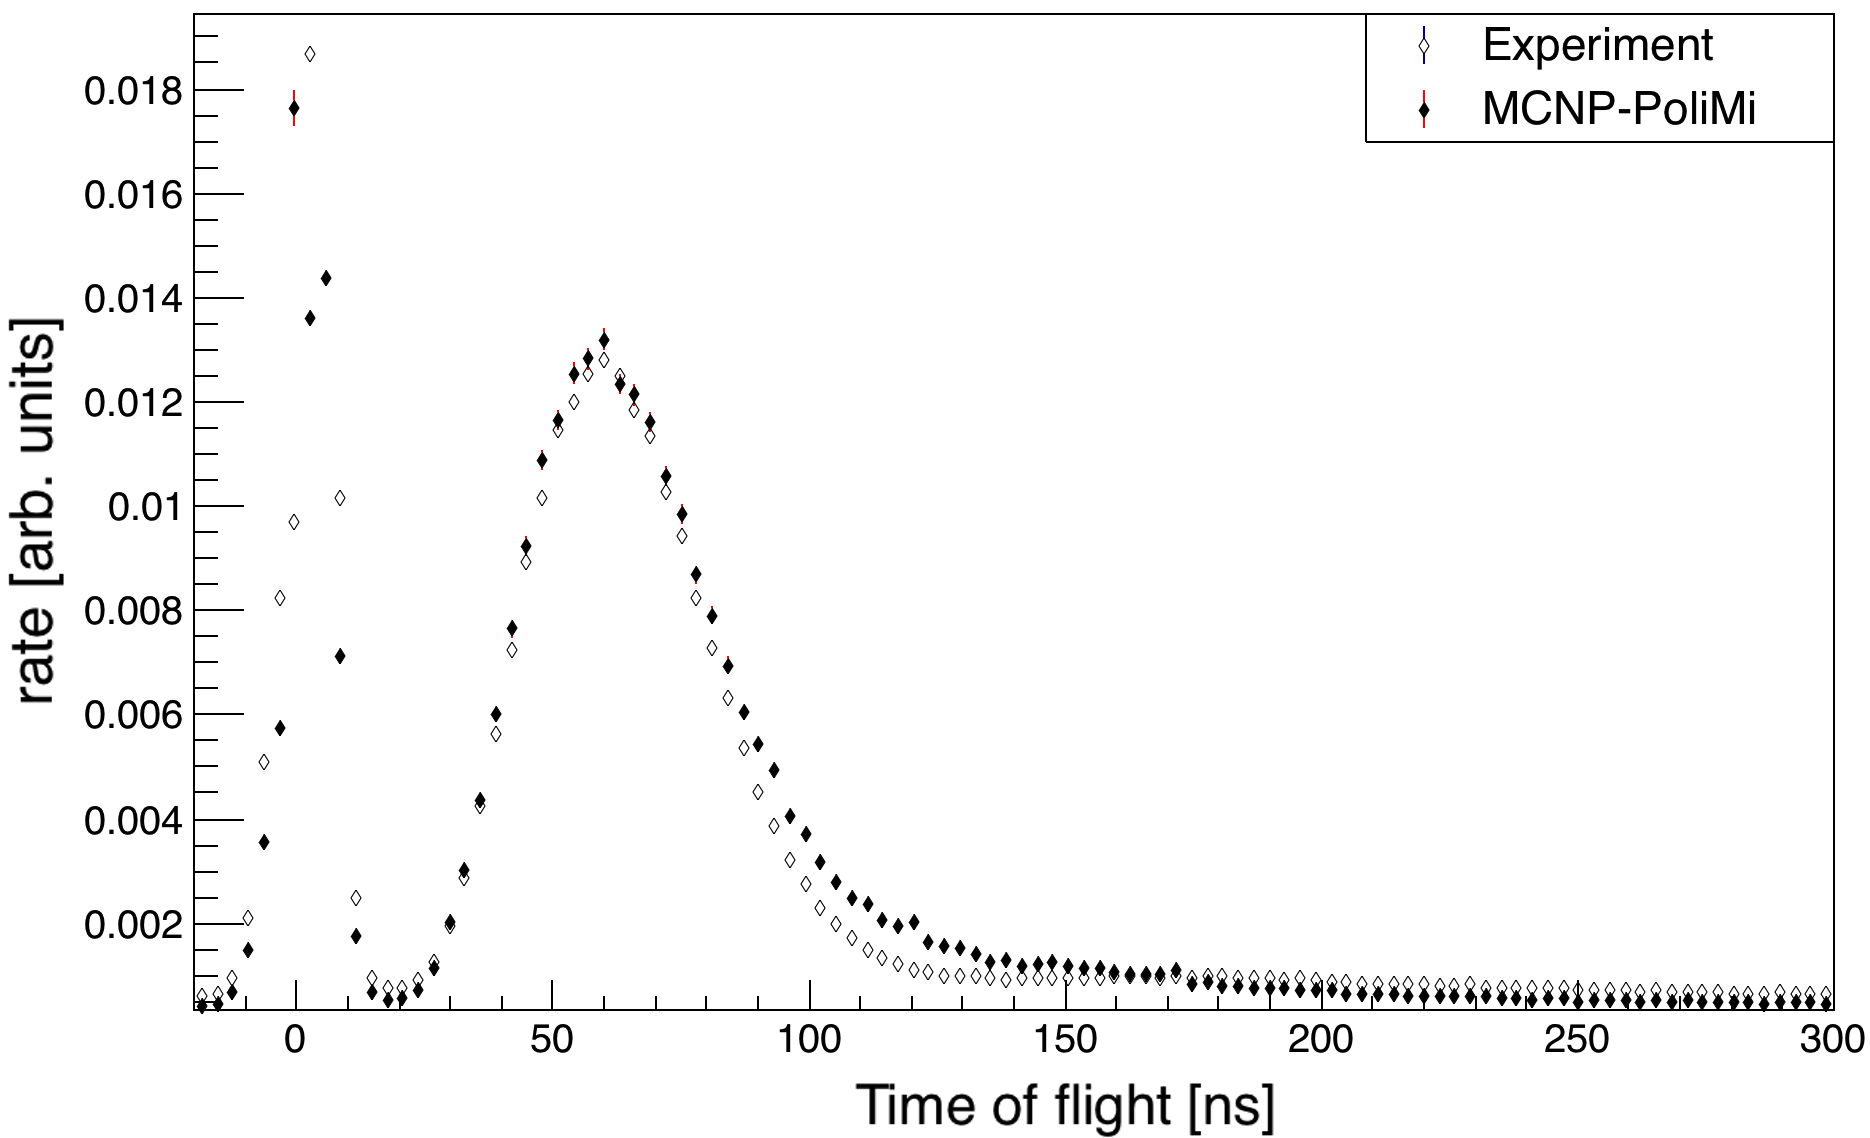
\includegraphics[width = \figsize\textwidth]{Cf252MCNPVsEXP.png}
    \caption{
    Measured versus simulated ToF spectrum from the SF of $^{252}$Cf.
    The simulation used the detector response model outlined in ref~\cite{MPPost}.
    The simulated and measured curves are normalized in order to facilitate comparison.
    }
    \label{fig:Cf252MCNPVsEXP}
\end{figure} % todo: line numbers 

Figure~\ref{fig:CrosstalkVScoincidence} shows the distribution of cross-talk events and true n-n coincidences as a function of reconstructed opening angle.
It is worth noting that, according to this simulation, the effect of cross-talk is not only small, but is also distributed over a wide range of angles rather than being concentrated around 0 degrees as one might expect.
Angles greater than 125 degrees are not shown in Fig.~\ref{fig:CrosstalkVScoincidence} because cross-talk events at large angles can be readily identified in analysis due to the large amount of time required for a neutron to travel these distances.
The simulation was initially performed with 5 cm of lead shielding placed behind the scintillators, and the number of cross-talk events accounted for 11\% of the total coincident neutron events.
This value fell to 3\% when polyethylene was used instead of lead, motivating the placement of 10~cm of polyethylene behind the detectors instead of lead.
\begin{figure}
    \centering
    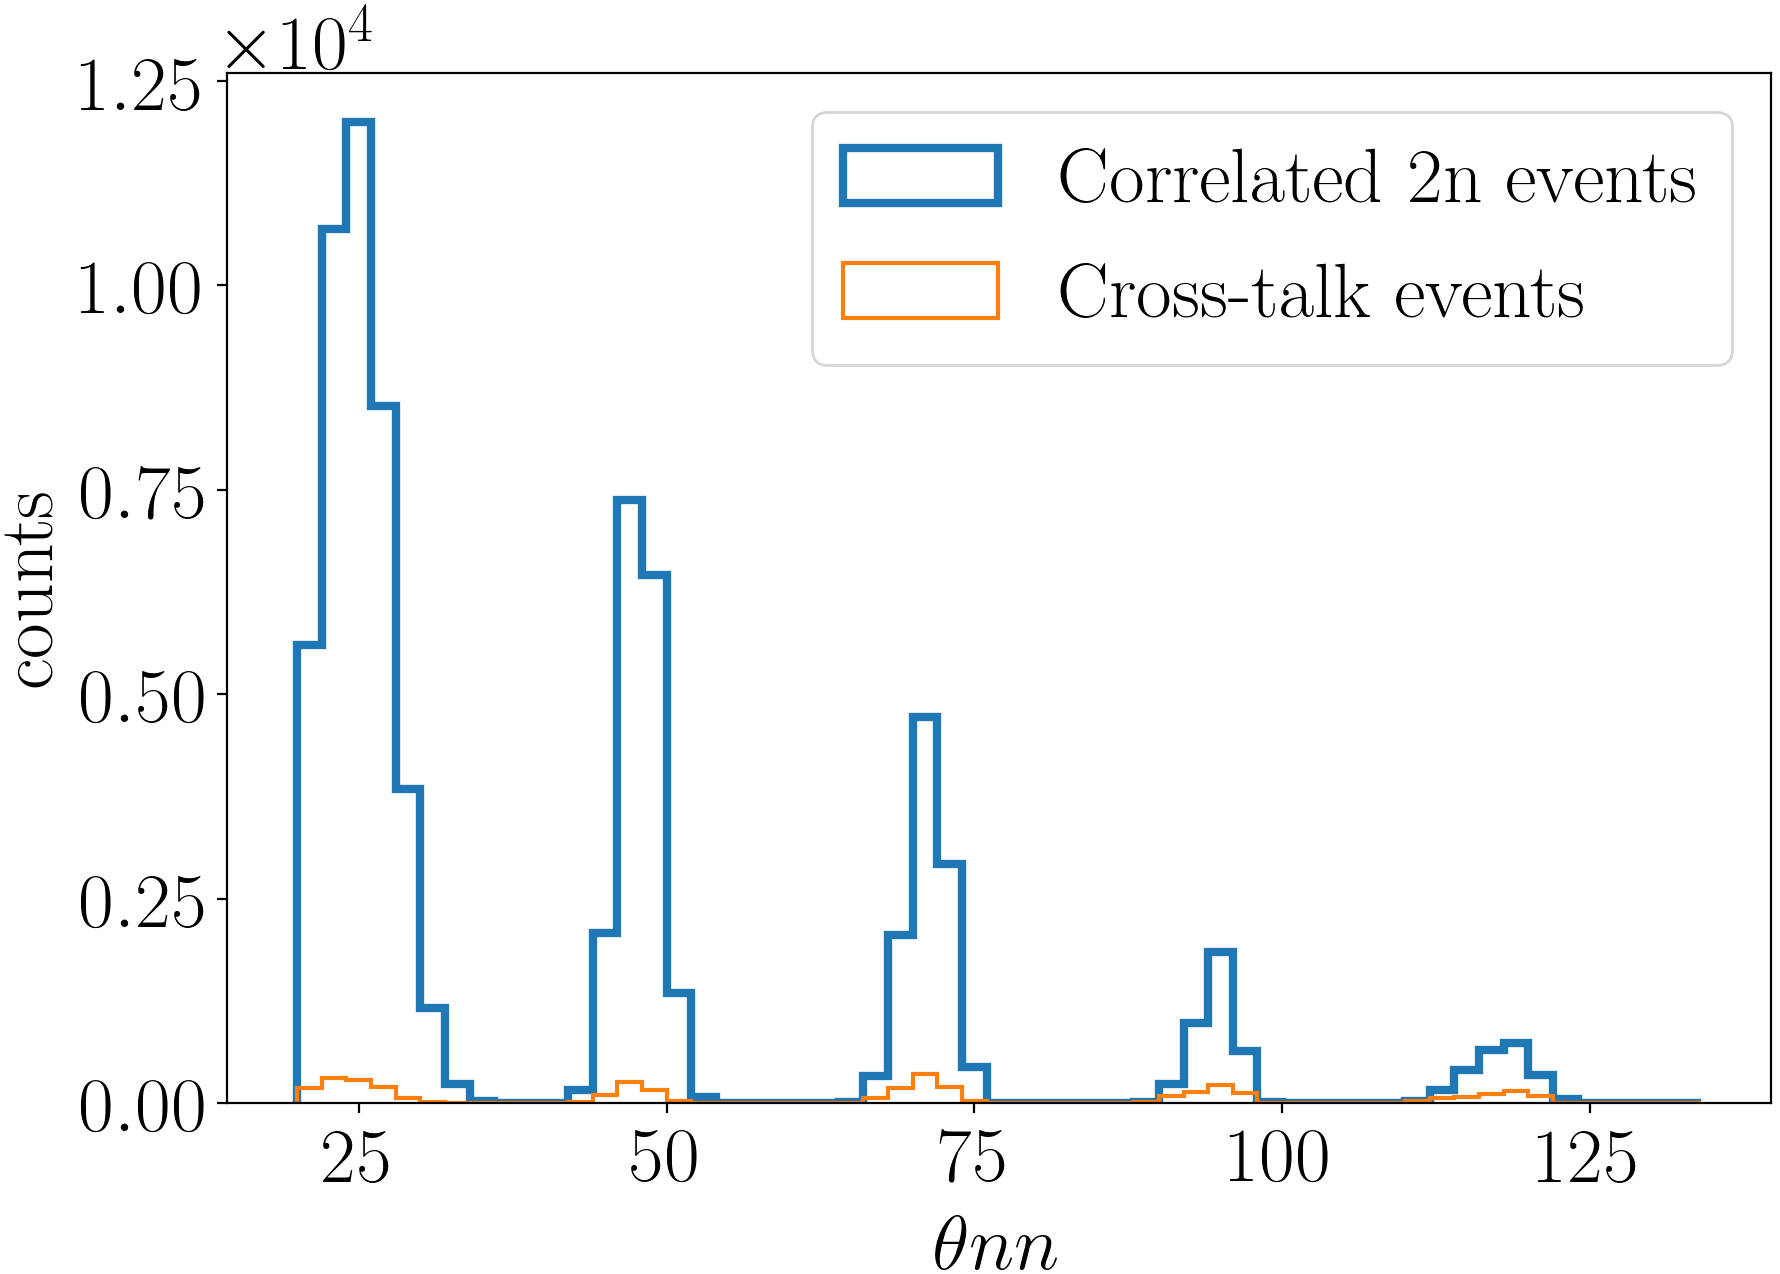
\includegraphics[width = \figsize\textwidth]{CrosstalkVScoincidence.png}
    \caption{
    MCNP-PoLiMi simulation of the number of cross-talk events versus correlated n-n events as a function of reconstructed opening angle.
    Cross-talk accounted for 3\% of total events.
    Simulated cross-talk events do not occur primarily at small angles, but are instead spread out over a wide range of angles.
    Any cross-talk occurring at angles larger than 125$^{\circ}$ will be removed from the experimental data by the cuts applied to neutron ToF.
    }
    \label{fig:CrosstalkVScoincidence}
\end{figure}

